\section{Results and Discussion}

The position probability densities can be seen in Figure~\ref{densities}. On the top, there's the longitudinal pump and on the bottom the transversal. The leftmost state is the first eigenstate, the second eigenstate is in the middle and the third on the right. The first eigenstate has the lowest energy. The solid blue lines represent the position probability densities, the dashed orange lines represent the potentials. The potential plot was created by taking the expressions of the respective Hamiltonians that act both on the atom part and the photon part of the composite system. For the operators the expectation values were taken. Each peak of the ground state density being located at the potential minima is in accordance with our expectations. Notice that the transversal position probability density is $\lambda / 2$-periodic despite the Hamiltonian being $\lambda$-periodic. This is because we're actually looking at the superposition of two symmetric states that are shifted by $\lambda / 2$. There'd be actually two potentials in Figure~\ref{trans_density}, one for each state. However, only one was chosen so that the graph doesn't get too confusing. The other potential would look the same, but shifted by $\lambda / 2$. The position probability densities give us an idea where the atoms are located. There are some properties of the systems, however, which still remain hidden to us in this representation. For that, we'll take a look at the momentum space.

\begin{figure}[!htb]
	\begin{minipage}[b]{1\linewidth}
	\centering
	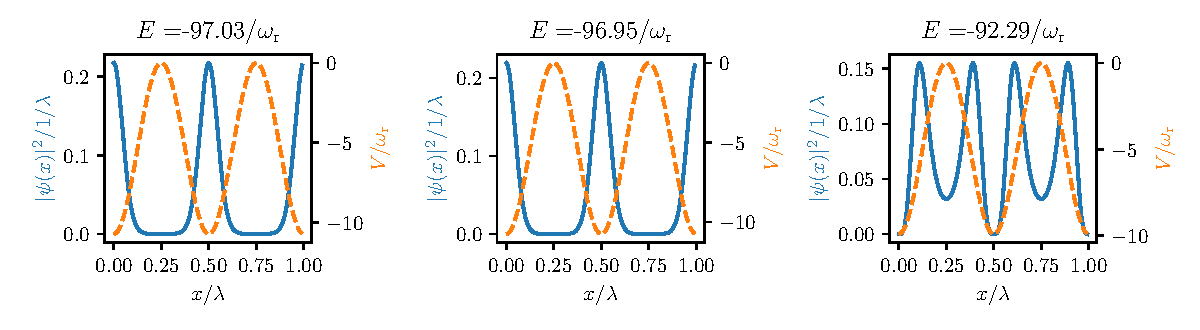
\includegraphics[width=1\textwidth]{images/dens_long.pdf}
	\subcaption{Longitudinal, $\eta = 30 \, \omega_\text{r}$.}
	\label{long_density}
	\end{minipage}
%
	\begin{minipage}[b]{1\linewidth}
	\centering
	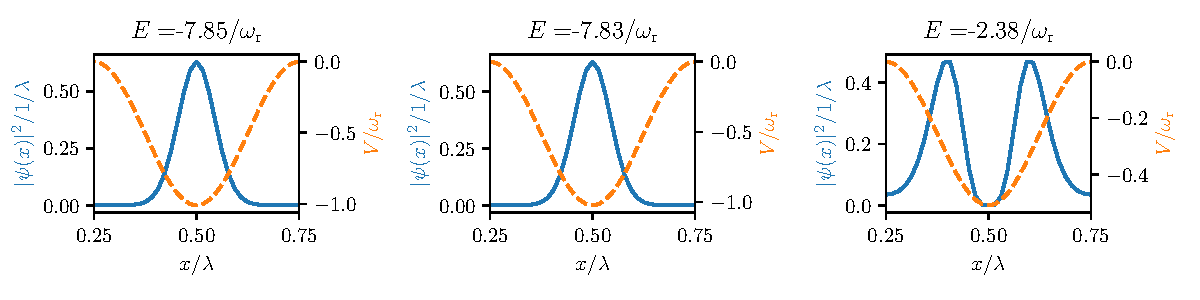
\includegraphics[width=1\textwidth]{images/dens_trans.pdf}
	\subcaption{Transversal, $\eta = 10 \, \omega_\text{r}$.}
	\label{trans_density}
	\end{minipage}
\caption{Longitudinal and transversal position probability densities. The solid blue lines represent the position probability densities and the dashed orange lines represent the potentials. The first eigenstate is on the left, the second in the middle and the third on the right. The wave function densities being located at potential minima meets our expectation. Note that the transversal position probability density appears to be $\lambda / 2$-periodic. That is because we're actually looking at the superposition of two symmetric states that are shifted by $\lambda / 2$.}
\label{densities}
\end{figure}
\FloatBarrier

\noindent The momentum distribution for different values of $\eta$ can be seen in Figure~\ref{momenta}. At $\eta = 0$, i.e. when the laser is off, there's only a peak at 0, meaning the atoms have no momentum. When we start pumping, we get other peaks than 0. Now the atoms do have momentum. For longitudinal pumping, there's always a gap between each peak which is not the case for transversal pumping. Take a look again at figure~\ref{pumping}. When we pump longitudinally, a photon is only able to transfer a momentum of $2 \hbar k$ because of momentum conservation. Thus we only observe peaks at $2n\hbar k$, where $n \in \mathbb{N}$. For transversal pumping, the same processes of photons transferring momenta of $2\hbar k$ are happening, but now we also have a momentum transfer of $\hbar k$ when a transversally incoming photon is being scattered into the cavity. Naturally, the more we pump, the more outer momenta we will get.

\begin{figure}[!htb]
	\begin{minipage}[b]{1\linewidth}
	\centering
	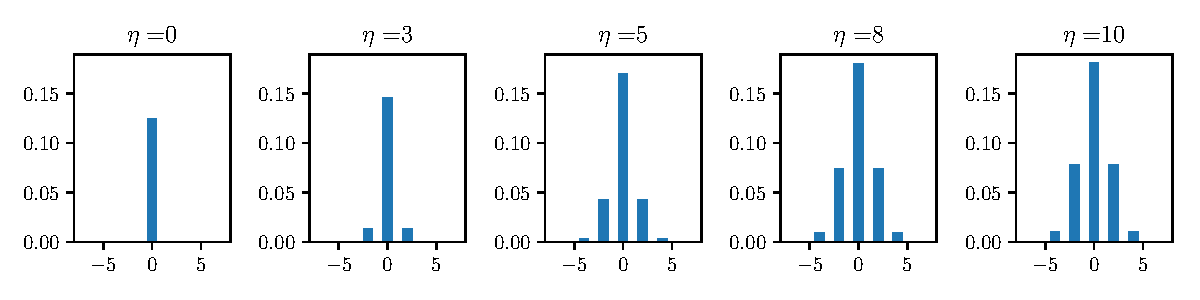
\includegraphics[width=1\textwidth]{images/mom_long.pdf}
	\subcaption{Longitudinal.}
	\label{long_momentum}
	\end{minipage}
%
	\begin{minipage}[b]{1\linewidth}
	\centering
	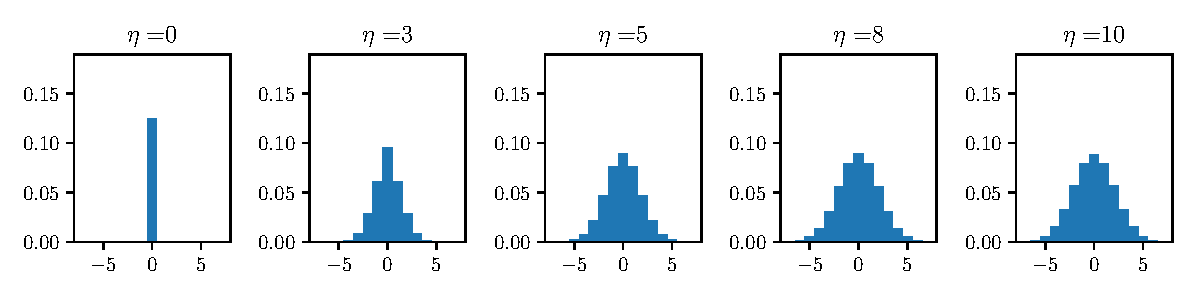
\includegraphics[width=1\textwidth]{images/mom_trans.pdf}
	\subcaption{Transversal.}
	\label{trans_momentum}
	\end{minipage}
\caption{Longitudinal and transversal momentum distributions. For longitudinal pump, there are only momenta of $2 n \hbar k$ because longitudinal scattering processes only allow momenta transfer of $2 \hbar k$. For transversal pump, there is no such restriction and we have momenta of $n \hbar k$.}
\label{momenta}
\end{figure}
\FloatBarrier

\noindent Having looked at the atom part of the composite system, let's take a look at the photon part. The photon number distribution for different values of $\eta$ can be seen in Figure~\ref{photon_dist}. The mean and variance are the same, thus we have a Poisson distribution.

\begin{figure}[!htb]
	\begin{minipage}[b]{1\linewidth}
	\centering
	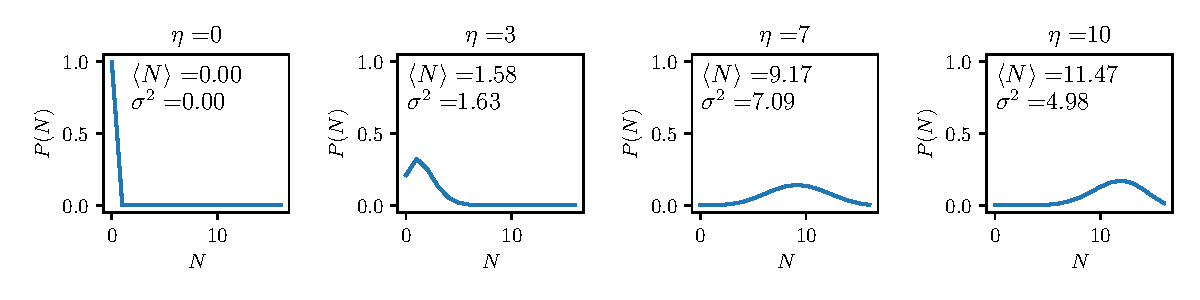
\includegraphics[width=1\textwidth]{images/pho_dens_long.pdf}
	\subcaption{Longitudinal.}
	\end{minipage}
%
	\begin{minipage}[b]{1\linewidth}
	\centering
	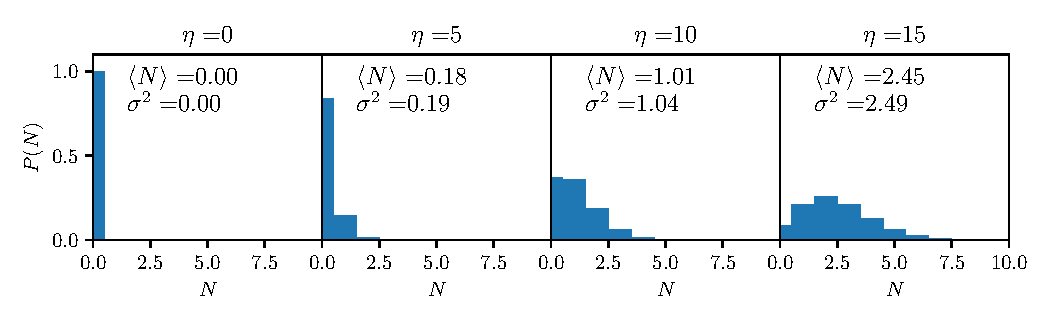
\includegraphics[width=1\textwidth]{images/pho_dens_trans.pdf}
	\subcaption{Transversal.}
	\end{minipage}
\caption{Longitudinal and transversal photon distributions. Since the mean and the variance are the same, we have a Poisson distribution.}
\label{photon_dist}
\end{figure}
\FloatBarrier

\noindent The Humsimi Q representation of the photon states for longitudinal and transversal pump can be seen in Figure~\ref{qfunc}. What we can see is a two-dimentional plane. A point on this plane represents a state the light field can be in. Remember that the state $| \alpha \rangle$ is represented by a complex number $\alpha = X + iP$. We don't only see a point, however, we can see a blob. That is because of the quantum uncertainty. The color represents the probability of a certain state, white is the hightest probability and black 0. Taking a look at the longitudinal case, the blob is initially at 0 meaning that there's no light field. There more we pump then, the higher the blob will move which indicates the emergence of a light field. A light field being present means of course the atoms being arranged in a lattice. For the transversal pump, the graphs look a little different. First of all, we can observe two blobs. That is because we're looking at the superposition of two symmetric states that we can't separate in the simulation. Then notice also that initially the blob in the middle doesn't separate into two, but stretches with the highest probability of the state still being at 0.


\begin{figure}[!htb]
	\begin{minipage}[b]{1\linewidth}
	\centering
	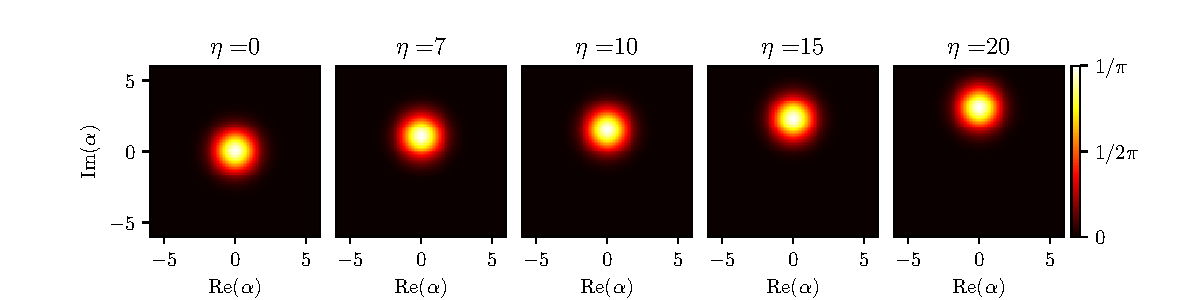
\includegraphics[width=1\textwidth]{images/qfunc_long.pdf}
	\subcaption{Longitudinal.}
	\end{minipage}
%
	\begin{minipage}[b]{1\linewidth}
	\centering
	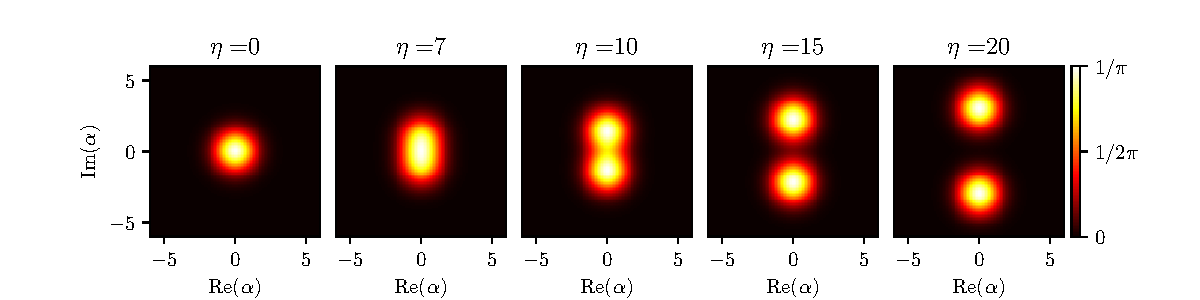
\includegraphics[width=1\textwidth]{images/qfunc_trans.pdf}
	\subcaption{Transversal.}
	\end{minipage}
\caption{Husimi Q representation of photon states for longitudinal and transversal pumping. A point in the plane represents a state $| \alpha \rangle$ of the light field and the color the probability of that state. Since there's quantum uncertainty, we don't observe a point but a blob. For transversal pumping, the blob initially doesn't move but only stretches. Only at sufficient pump strengths, the blob will move and thus a light field build up. Observing two blobs for transversal pumping means we're actually looking at the superposition of two symmetric states.}
\label{qfunc}
\end{figure}
\FloatBarrier

\noindent We can visualize the fact that the two blobs initially don't separate but only stretch by plotting the pump parameter $\eta$ on the $x$-axis and the most likely state for one half of the plane on the $y$-axis which is effectively the absolute value of $\alpha$. We can see the result at Figure~\ref{fig_order_param}. For longitudinal pumping, the more we pump, the more light field will build up, i.e. there is a direct relationship between pumping and light field intensity. For transversal pumping we can see another picture, however. Initially when we pump, the graph stays at 0 meaning no light field is building up. Only at a critical pump strength, a light-field will suddenly emerge. This is what we have discussed earlier about the sudden face transition for the transversal pumping.

\begin{figure}[!htb]
	\begin{minipage}[b]{.5\linewidth}
	\centering
	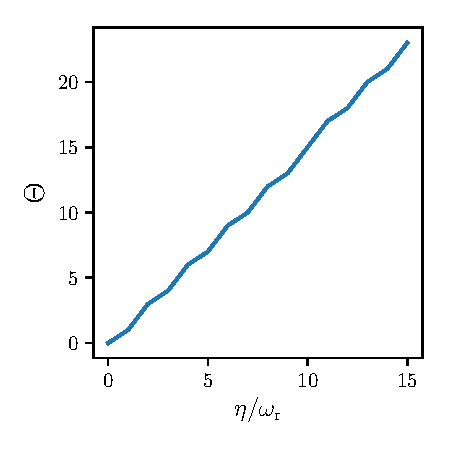
\includegraphics[width=.9\textwidth]{images/theta_long.pdf}
	\subcaption{Longitudinal.}
	\end{minipage}
%
	\begin{minipage}[b]{.5\linewidth}
	\centering
	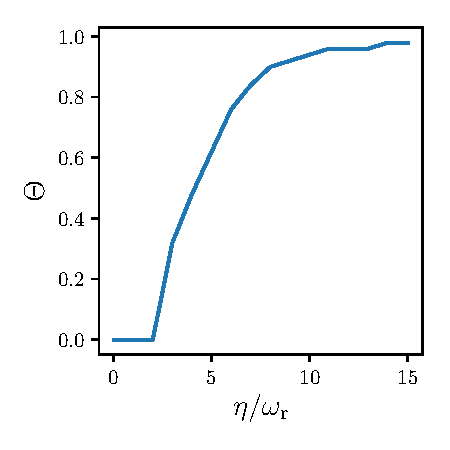
\includegraphics[width=.9\textwidth]{images/theta_trans.pdf}
	\subcaption{Transversal.}
	\end{minipage}
\caption{Most likely value of the photon state momentum looking at only the positive side of the phase space for longitudinal and transversal pumping. For longitudinal pumping, the momentum increases gradually. For transversal pumping, the light initially does not gain any momentum, meaning that the atoms resist being in order. At a critical pump strength, a light field suddenly builds up and the atoms self-order.}
\label{fig_order_param}
\end{figure}
\FloatBarrier

\noindent The more we pump, the more photons will appear. We have to take that into account by raising the maximum amount of allowed photon states $N_\text{cutoff}$. Raising $N_\text{cutoff}$ results in longer simulation times which can be bothersome. However, if we don't do so, our results become faulty. Take a look at Figure~\ref{model_limit} which depicts the photon number distributions for longitudinal pump for different values of $N_\text{cutoff}$ at $\eta = 40 \, \omega_\text{r}$. For our parameters, $40 \, \omega_\text{r}$ is a relatively high value for $\eta$ and we thus would expect a high average photon number which we cannot possibly obtain if we limit $N_\text{cutoff}$ to 8. To check the validity of our results, i.e. if $N_\text{cutoff}$ is set high enough, we can look at the standard deviation. For a Poisson distribution, the mean has to be the same as the standard deviation which is not the case if we set the cutoff too low.

\begin{figure}[!htb]
	\centering
	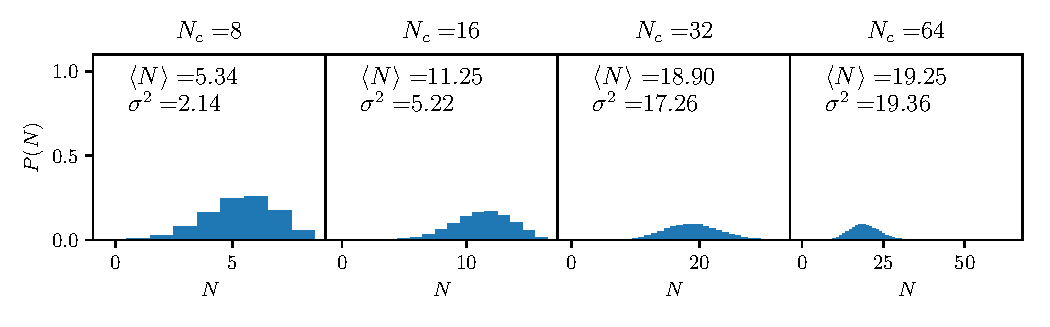
\includegraphics[width=1\textwidth]{images/model_limit_long.pdf}
	\caption{Photon number distributions for longitudinal pump for different values of $N_\text{cutoff}$ at $\eta = 40 \, \omega_\text{r}$. If we don't set $N_\text{cutoff}$ sufficiently high, we get bogus results. A quick sanity check is to compare the mean with the variance. For a Poisson distribution, they have to be the same.}
	\label{model_limit}
\end{figure}
\FloatBarrier
